\section{统一热-质耦合输运模型}
\label{sec:model}

四问共用一套控制方程、一套坐标与一套离散格式。本节把它们集中推导一次：
先从能量与水分守恒出发确定方程形式，再引入干质量坐标把收缩问题化为定域问题，
最后给出使边界条件以原始形式进入方程组的离散格式。此后各问只需交代物性闭合、
几何条件与终止判据的差别。

\subsection{几何降维与守恒起点}

药材近似为长 $25$ cm、半径 $2$ cm 的圆柱，长径比 $L/R_0=12.5$。
侧面积 $2\pi R_0L=0.0314$ m$^2$ 是两端面积 $2\pi R_0^2=0.0025$ m$^2$ 的 $12.5$ 倍，
端面仅占总换热面积的 $7.4\%$。另一条依据来自题面的输出格式：制表只以
“到药材中心的距离”一个坐标索引，若保留轴向坐标，同一半径不同高度处的
温度与含水率并不相同，一个半径将对应一族数值而非一个数值。
需要说明这只是本文的建模取舍，不是物理上的必然：轴向梯度在端面附近客观存在，
面积占比 $7.4\%$ 给出的是其影响的量级上界，而非证明其可忽略；
量化该偏差需要二维轴对称计算，本文未做，
故只在第~\ref{sec:validation}~节给出偏差方向（时长偏长）而不给幅度。
在此前提下忽略轴向与周向输运，把问题降为一维径向轴对称。

\begin{figure}[!htbp]
  \centering
  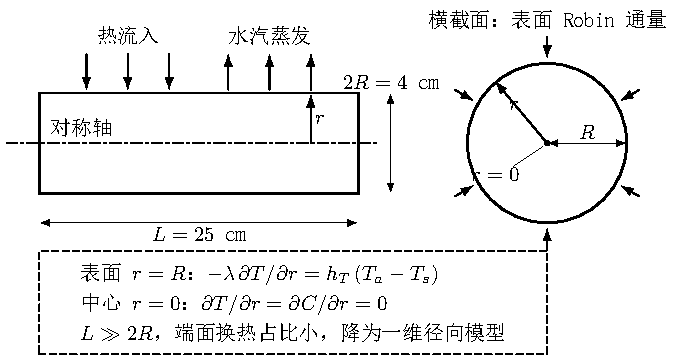
\includegraphics[width=0.9\textwidth,height=0.8\textheight,keepaspectratio]{../figures/tikz_cylinder_geometry.pdf}
  \caption{圆柱几何与边界条件}
  \label{fig:cylinder_geometry}
\end{figure}

降维后仅存两个通量方向，且二者相反：热量由热风经侧面传入、向轴心推进，
水分由内部向侧面迁移、再被气流带走（图~\ref{fig:cylinder_geometry}~标出这两个方向
与轴心、侧面两处边界）。
这一点在后文解释“表面先干、中心后干”与“表面先热、中心后热”
为何在时间尺度上差异悬殊时会多次用到。轴心处由对称性给出零通量条件，
它替代了通常意义上的第二个边界。

在半径 $r$ 处取厚度 $\mathrm{d}r$ 的环状控制体，对其写能量守恒：
单位时间内温度升高所需热量等于净流入的导热热量。以 $\rho(C)$、$c_p(C)$、$k(C)$
分别记密度、比热容与热传导系数，得

\begin{equation}
\rho(C)c_p(C)\frac{\partial T}{\partial t}
=\frac{1}{r}\frac{\partial}{\partial r}\!\left(r\,k(C)\frac{\partial T}{\partial r}\right),
\qquad 0<r<R(t).
\label{eq:heat_phys}
\end{equation}

水分一侧按假设（2）取 Fick 定律，以干基含水率 $C$ 为输运变量，
扩散系数 $D(C,T)$ 由附录经验式闭合：

\begin{equation}
\frac{\partial C}{\partial t}
=\frac{1}{r}\frac{\partial}{\partial r}\!\left(r\,D(C,T)\frac{\partial C}{\partial r}\right),
\qquad 0<r<R(t).
\label{eq:mass_phys}
\end{equation}

式~\eqref{eq:heat_phys}~与~\eqref{eq:mass_phys}~通过 $D$ 对 $T$ 的依赖
以及 $\rho,c_p,k$ 对 $C$ 的依赖双向耦合，只有在附录 2 的常物性闭合下
温度方程才退化为线性。

\subsection{边界条件与传递驱动力}

轴心处对称性给出

\begin{equation}
\left.\frac{\partial T}{\partial r}\right|_{r=0}=0,
\qquad
\left.\frac{\partial C}{\partial r}\right|_{r=0}=0.
\label{eq:axis_bc}
\end{equation}

表面处热、质均按对流规律传递。热 Biot 数 $hR_0/k=25\times0.02/0.36=1.3889$
落在内外热阻相当的区间：既不能把药材视为温度均匀的集中参数体
（那要求 $Bi\ll1$），也不能把表面温度直接钉在热风温度上（那要求 $Bi\gg1$），
必须采用第三类边界条件。初始含水率下扩散系数约 $4.94\times10^{-9}$ m$^2$/s，
对应质 Biot 数 $h_mR_0/D\approx3.24$，同样两侧阻力均不可忽略。于是

\begin{equation}
-k(C)\left.\frac{\partial T}{\partial r}\right|_{r=R}
=h\left[T(R,t)-T_{\mathrm{air}}(t)\right],
\qquad
-D(C,T)\left.\frac{\partial C}{\partial r}\right|_{r=R}
=h_m\left[C(R,t)-W_{\mathrm{air}}(t)\right].
\label{eq:surface_bc}
\end{equation}

这一对边界条件即固体与周围介质间热质交换的标准形式\upcite{luikov1966surface}。
式~\eqref{eq:surface_bc}~右端的传质驱动力直接取空气含湿量
$W_{\mathrm{air}}(t)$，而非通常做法中的平衡含水率 $C_{\mathrm{eq}}$。
理由是引入 $C_{\mathrm{eq}}$ 必须给出吸附等温线，而题面与附录均未提供，
自拟等温线等于向模型注入题面之外的自由参数。这一读法还有一个必要的后果：
$W_{\mathrm{air}}$ 的平台值约 $0.05$ kg/kg，低于烘干阈值 $0.15$ kg/kg，
因此阈值必定在有限时间内达到，问题三与问题四的解存在。
若表面驱动浓度高于阈值，无论烘多久都不可能达标，题设本身就会失去意义。

初始条件由题面直接给出，$T(r,0)=28$ °C、$C(r,0)=2.55$ kg/kg，两者沿半径均匀。

\subsection{烘房条件与边界驱动数据}

式~\eqref{eq:surface_bc}~中的 $T_{\mathrm{air}}(t)$ 与 $W_{\mathrm{air}}(t)$
由附件 1 给出，覆盖 $0$ 至 $14400$ s、间隔 $60$ s 共 $241$ 个点，
中间时刻按线性插值取用。

\begin{figure}[!htbp]
  \centering
  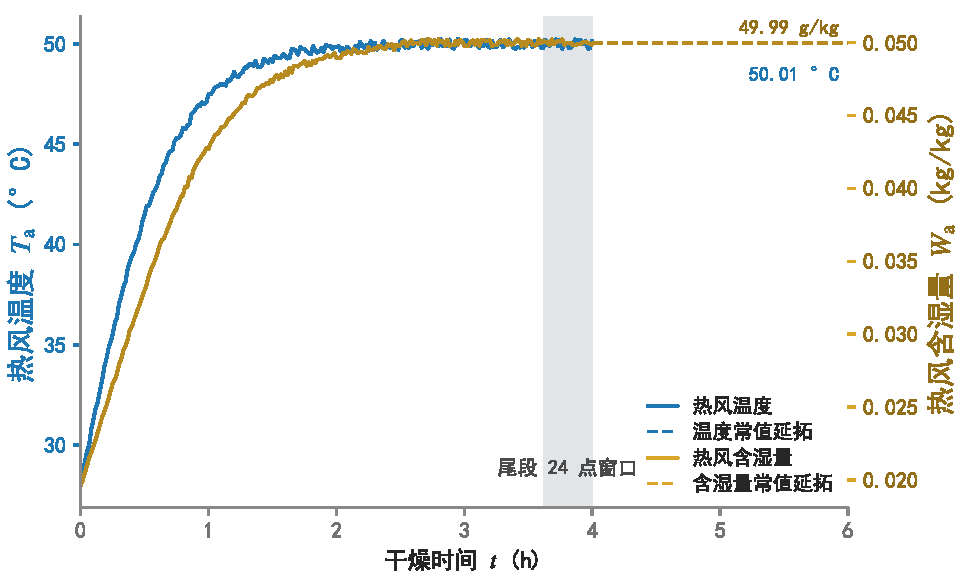
\includegraphics[width=0.9\textwidth,height=0.8\textheight,keepaspectratio]{../figures/fig_air_condition.pdf}
  \caption{热风温度与含湿量时程}
  \label{fig:air_condition}
\end{figure}

热风温度与含湿量两条曲线在约 $6000$ s 后都进入平台（图~\ref{fig:air_condition}）。
末 $24$ 个点的温度均值为 $50.0095$ °C、含湿量均值为 $0.049986$ kg/kg，
温度波动收在 $\pm0.26$ °C 以内；该段的线性拟合斜率仅 $0.06$ °C/h、
全段累计变化 $0.02$ °C，说明摆动是无趋势的随机散布而非残余升温。
问题三与问题四所需的时间跨度达五十余小时，远超附件 1 的覆盖范围，
故 $t>14400$ s 之后取上述均值作常数延拓。取均值而非末点，
是因为均值能抑制单点测量波动；取常数而非趋势外推，
是因为“恒温干燥”的字面含义就是此后烘房条件不再变化。

需要在结果之前就交代清楚的是这一延拓的权重：问题三 $57.4247$ h 的总时长中，
附件 1 实测覆盖的仅前 $4$ h，其余约 $93\%$ 的时间轴由延拓段支配。
第~\ref{sec:validation}~节的灵敏度分析给出该依赖的定量边界——
平台温度改变 $\pm0.5$ °C，烘干时长反向变化约 $1.6\%$，
折合约 $0.9$ h。因此本文给出的烘干时长应理解为“在恒温平台取该均值前提下”的
结果，而非无条件的绝对值。

两个附件提供的三条输入序列汇总于表~\ref{tab:input_stats}，
它们是本文全部边界条件与几何输入的唯一来源。

\begin{table}[H]
  \centering
  \caption{附件输入数据描述性统计}
  \label{tab:input_stats}
  \setlength{\tabcolsep}{4pt}
  \begin{tabular}{lrrrl}
  \toprule
  输入序列 & 样本数 & 起始或 $3$ h 值 & 末段代表值 & 末段值的取法 \\
  \midrule
  附件 1 热风温度 (°C)        & 241 & 50.1950 & 50.0095 & $13020$ s 后各点均值 \\
  附件 1 热风含湿量 (kg/kg)   & 241 & 0.04977 & 0.04999 & $13020$ s 后各点均值 \\
  附件 2 药材半径 (cm)        & 145 & 2.000   & 1.198   & 全程最小半径 \\
  \bottomrule
  \end{tabular}
\end{table}

表~\ref{tab:input_stats}~中附件 1 两行的“末段代表值”即上文用于常数延拓的平台均值，
$3$ h 处取值与之相差不足 $0.19$ °C 与 $0.0003$ kg/kg，
可见平台在附件 1 覆盖范围内已经建立，延拓并非把上升段的趋势外推出去。
附件 2 一行的取法不同：半径全程单调收缩，故第三列列出的是初值 $2.000$ cm、
末列为全程最小值 $1.198$ cm，中途 $6$ h 处为 $1.374$ cm，
其完整形态与对烘干时长的影响留到第~\ref{sec:p4}~节讨论。
三条序列的采样间隔分别为 $60$ s、$60$ s 与 $1800$ s，
中间时刻一律按线性插值取用，不做平滑或重采样。

\subsection{干质量拉格朗日坐标}

问题四中外半径 $R(t)$ 随时间收缩，物理域是移动边界问题。
若直接在 $r$ 上离散，网格须随时间重排，且方程中会出现网格运动带来的
伪对流项。规避这一困难的通行做法是把动边界映射到固定域上，
再以单个几何因子承载收缩\upcite{adrover2019shortcut}。本文改用干质量坐标

\begin{equation}
s=\left(\frac{r}{R(t)}\right)^{2}\in[0,1].
\label{eq:coord_def}
\end{equation}

选择平方而非线性比值，是因为 $s$ 正比于横截面积、从而正比于该半径以内包含的
干物质量。在假设（4）的仿射收缩下，每个物质点的 $r/R(t)$ 保持不变，
故每个 $s$ 值始终标记同一批干物质，坐标本身即拉格朗日坐标。

\begin{figure}[!htbp]
  \centering
  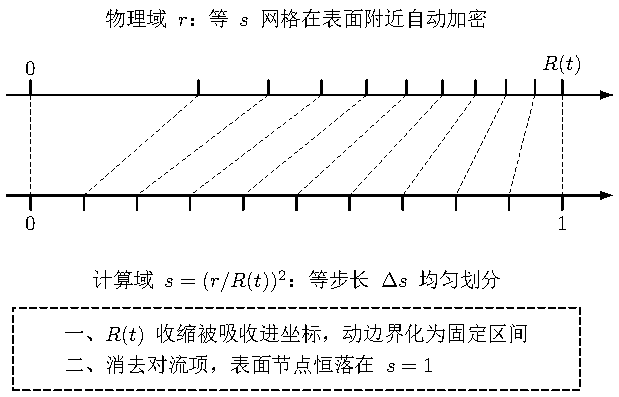
\includegraphics[width=0.9\textwidth,height=0.8\textheight,keepaspectratio]{../figures/tikz_coord_mapping.pdf}
  \caption{干质量坐标映射关系}
  \label{fig:coord_mapping}
\end{figure}

这一映射还带来两个附带好处（图~\ref{fig:coord_mapping}）。
其一，均匀的 $s$ 网格在物理空间自动向表面加密——表面正是浓度梯度最陡、
Robin 条件最需要分辨的位置；其二，$R(t)$ 收缩时全部节点随边界等比例内移，
网格拓扑不变。

设干骨架密度为 $\rho_s$。干物质总量守恒要求
$\rho_s(t)\pi R(t)^2L=\rho_{s0}\pi R_0^2L$，即

\begin{equation}
\rho_s(t)=\rho_{s0}\left(\frac{R_0}{R(t)}\right)^{2}.
\label{eq:rho_s}
\end{equation}

半径以内的干质量 $M_s(s)=\rho_s(t)\pi R(t)^2Ls=\rho_{s0}\pi R_0^2Ls$
与时间无关，这正是把 $s$ 用作输运坐标的依据。
由 $r=R\sqrt{s}$ 计算 $\partial/\partial r=(2\sqrt{s}/R)\partial/\partial s$
并代入式~\eqref{eq:mass_phys}，注意固定 $s$ 求时间导数时收缩项已被坐标吸收，
得到

\begin{equation}
\left.\frac{\partial C}{\partial t}\right|_{s}
=\frac{4}{R(t)^{2}}\frac{\partial}{\partial s}
\left(s\,D(C,T)\frac{\partial C}{\partial s}\right).
\label{eq:mass_s}
\end{equation}

温度方程作同样变换：

\begin{equation}
\rho(C)c_p(C)\left.\frac{\partial T}{\partial t}\right|_{s}
=\frac{4}{R(t)^{2}}\frac{\partial}{\partial s}
\left(s\,k(C)\frac{\partial T}{\partial s}\right).
\label{eq:heat_s}
\end{equation}

式~\eqref{eq:mass_s}~与~\eqref{eq:heat_s}~有三个值得指出的性质。
收缩在方程内部只留下系数 $4/R(t)^2$ 一处，不产生任何伪对流项
（$R(t)$ 另出现在下文式~\eqref{eq:bc_s}~的表面通量系数中，
两处都是随时间已知的标量因子，不引入新的微分项）；
柱坐标在 $r=0$ 处的 $1/r$ 奇点被 $s$ 因子吸收，轴心不再需要特殊处理；
求解域恒为 $[0,1]$，问题一至问题三取 $R\equiv R_0$ 即为定域情形，
四问因此可以共用同一份求解器。

边界条件随之改写。$s=0$ 处 $s\,\partial C/\partial s\to0$ 自动满足对称性，
$s=1$ 处由 $\partial/\partial r=(2/R)\partial/\partial s$ 得

\begin{equation}
-\frac{2k}{R}\left.\frac{\partial T}{\partial s}\right|_{s=1}
=h\left(T_R-T_{\mathrm{air}}\right),
\qquad
-\frac{2D}{R}\left.\frac{\partial C}{\partial s}\right|_{s=1}
=h_m\left(C_R-W_{\mathrm{air}}\right).
\label{eq:bc_s}
\end{equation}

对式~\eqref{eq:mass_s}~在 $[0,1]$ 上积分并代入式~\eqref{eq:bc_s}，
得到干质量加权平均含水率 $\bar C=\int_0^1C\,\mathrm{d}s$ 的全局平衡关系

\begin{equation}
\frac{\mathrm{d}\bar C}{\mathrm{d}t}
=-\frac{2h_m}{R(t)}\left(C_R-W_{\mathrm{air}}\right).
\label{eq:global_balance}
\end{equation}

式~\eqref{eq:global_balance}~不参与求解，但提供了一个与离散格式无关的
守恒检验：数值解的 $\bar C$ 变化率必须与表面通量逐步吻合。
第~\ref{sec:validation}~节用它给出的残差量级为 $10^{-10}$。

\subsection{节点中心有限体积离散}

在均匀 $s$ 网格上对散度形式方程作节点中心有限体积离散，内部节点由相邻界面通量差更新；轴心自然为零通量，表面半控制体直接装配 Robin 通量。后向 Euler 配合三次 Picard 迭代形成三对角方程组。该格式守恒且使表面值保持原始未知量；完整通量、端点半控制体推导见附录 B。
\iffalse

上述两个控制方程都是散度形式的非线性扩散方程，有限体积离散能逐个控制体地
满足守恒，正适合这类物性随解变化的问题\upcite{zhang2022fv}。
把 $[0,1]$ 划分为 $N$ 个等距区间，
节点 $s_i=i\Delta s$，$i=0,\dots,N$，
$\Delta s=1/N$。控制体以节点为中心：内部节点的控制体测度为 $\Delta s$，
两端节点为半格 $\Delta s/2$。

\begin{figure}[!htbp]
  \centering
  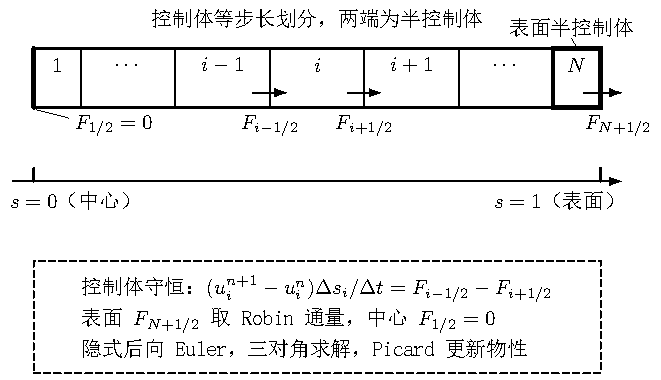
\includegraphics[width=0.9\textwidth,height=0.8\textheight,keepaspectratio]{../figures/tikz_fv_stencil.pdf}
  \caption{有限体积控制体与通量}
  \label{fig:fv_stencil}
\end{figure}

端点取半格是本格式的关键（图~\ref{fig:fv_stencil}）。表面值 $C_N$ 因此是
一个原始未知量而非插值得到的辅助量，Robin 条件直接写在 $s=1$ 上，
不需要虚拟节点或外推。若改用格心格式，表面落在控制体边界之外，
Robin 条件只能一阶近似，代价是可观的：$N=160$ 时格心格式的网格收敛残差
问题三停在 $1.046\times10^{-3}$、问题四停在 $7.424\times10^{-4}$，
均无法满足本文设定的 $5\times10^{-4}$ 相邻相对差判据；
换用节点中心格式后，同一网格上两问残差分别降到 $3.602\times10^{-4}$
与 $7.919\times10^{-5}$，无须靠加密网格硬压。

界面 $s_{i+1/2}=(i+1/2)\Delta s$ 处的扩散通量取相邻节点物性的算术平均

\begin{equation}
G_{i+1/2}=s_{i+1/2}\,D_{i+1/2}\,\frac{C_{i+1}-C_{i}}{\Delta s},
\qquad
D_{i+1/2}=\tfrac{1}{2}\left(D_i+D_{i+1}\right).
\label{eq:flux}
\end{equation}

对内部节点的控制体作平衡，得

\begin{equation}
\Delta s\,\frac{\mathrm{d}C_i}{\mathrm{d}t}
=\frac{4}{R^{2}}\left(G_{i+1/2}-G_{i-1/2}\right),
\qquad i=1,\dots,N-1.
\label{eq:fv_inner}
\end{equation}

轴心节点的控制体为 $[0,\Delta s/2]$，其内侧界面处 $s_{1/2}$ 因子使通量
自动为零量级，无须额外条件：

\begin{equation}
\frac{\Delta s}{2}\frac{\mathrm{d}C_0}{\mathrm{d}t}
=\frac{4}{R^{2}}G_{1/2}.
\label{eq:fv_axis}
\end{equation}

表面节点的控制体为 $[1-\Delta s/2,1]$，外侧界面即物理表面，
其通量由式~\eqref{eq:bc_s}~给出的 $-(h_mR/2)(C_N-W_{\mathrm{air}})$ 代入，
连同 $4/R^2$ 与 $s=1$ 整理后为

\begin{equation}
\frac{\Delta s}{2}\frac{\mathrm{d}C_N}{\mathrm{d}t}
=-\frac{4}{R^{2}}G_{N-1/2}-\frac{2h_m}{R}\left(C_N-W_{\mathrm{air}}\right).
\label{eq:fv_surface}
\end{equation}

式~\eqref{eq:fv_surface}~表明 Robin 系数以 $2h_m/R$ 的形式
直接进入系数矩阵的对角元，其与 $W_{\mathrm{air}}$ 的乘积
则进入右端项。因此边界条件是按其原始形式代入的，无需借助虚拟节点外推，
不引入额外的边界近似；控制体内部的通量 $G_{N-1/2}$ 仍带有与内节点同阶的
截断误差。温度方程的离散完全平行：把式~\eqref{eq:flux}~至
\eqref{eq:fv_surface}~中的 $D$ 换成 $k$、$h_m$ 换成 $h$、$W_{\mathrm{air}}$
换成 $T_{\mathrm{air}}$，并在时间导数项前保留因子 $\rho(C)c_p(C)$ 即可。

\fi
\subsection{时间推进与非线性处理}

物性依赖解本身，方程是非线性的。显式格式在 $\Delta s$ 加密时稳定性条件
过于苛刻，故采用后向 Euler 隐式格式\upcite{cruz2019implicit}——它对系数
冻结后的线性问题无条件稳定，非线性情形下的稳定性不由此自动保证，
需由下文的时间步无关性检验实测确认——并以 Picard 迭代处理非线性：
每个时间步内先用上一迭代的温度更新水分场，再用更新后的含水率求解温度场，
顺序迭代三次。三次的依据是第三次迭代引起的相对变化已不影响结果的第四位小数，
即不改变本文各表的制表精度；这是按制表位数选定的实用停止准则，
而非收敛到浮点精度极限的断言。

离散后系数矩阵为三对角，用带状直接解法求解，单步计算量与 $N$ 成正比。
生产算例取 $N=160$。这个数选取自两个约束的交集：网格无关性要求
相邻加密的 $t_{\mathrm{dry}}$ 相对差小于 $5\times10^{-4}$，
而制表要求 $r=0$、$0.5$、$1$、$1.5$、$2$ cm 五个位置恰好落在节点上。
后一条要求 $N$ 是 $16$ 的倍数：由式~\eqref{eq:coord_def}，
这五个半径对应 $s=0$、$0.0625$、$0.25$、$0.5625$、$1$，
分母最大为 $16$。$N=160$ 同时满足两者，制表值全部为节点原值、
不含任何空间插值误差。

时间步长按各问的制表分辨率取值：问题一的 $1800$ s 预热段取
$\Delta t=0.25$ s，问题二的 $3$ h 算例取 $0.5$ s，
问题三与问题四的数十小时全过程算例取 $1$ s。
第~\ref{sec:validation}~节的时间步无关性检验表明 $\Delta t$ 由 $4$ s
减到 $0.5$ s 时 $t_{\mathrm{dry}}$ 仅变化 $3\times10^{-3}$ h。

\subsection{烘干时长的判定}

问题三与问题四要求的不是给定时刻的场，而是满足烘干要求的首个时刻。
题面“各处的水分浓度应低于 $0.15$ kg/kg”作用在空间最大值上，故

\begin{equation}
t_{\mathrm{dry}}=\min\left\{t:\ \max_{0\le r\le R(t)}C(r,t)<C_{\mathrm{th}}\right\},
\qquad C_{\mathrm{th}}=0.15~\text{kg/kg}.
\label{eq:tdry_def}
\end{equation}

式~\eqref{eq:tdry_def}~写在物理坐标 $r$ 上，与题面的表述一致；
由于 $r=R(t)\sqrt{s}$ 在 $[0,R(t)]$ 与 $[0,1]$ 之间是双射，
对 $r$ 取最大值与对求解坐标 $s$ 取最大值给出同一个值，
程序在 $s$ 网格上扫描即可，本文两种写法可互换使用。
该最大值直接使用需在每个输出步扫描全域。
本文所有算例的含水率剖面均沿半径单调递减：初始场均匀，表面是唯一的水分出口，
故内部含水率不低于外部；第~\ref{sec:validation}~节实测的最大正向径向梯度为
$2.22\times10^{-15}$，与浮点舍入同量级，未出现方向相反的梯度。
在此单调性成立的前提下空间最大值取于中心，式~\eqref{eq:tdry_def}~可标量化为
$C(0,t)<C_{\mathrm{th}}$。这一标量化依据的是各算例的实测单调性，
而非对任意参数组合成立的证明；程序仍按全域最大值判定，
单调性只用于解释为何两者给出相同结果。设输出步 $t_j$ 与 $t_{j+1}$ 分别位于阈值两侧，
按线性插值定位

\begin{equation}
t_{\mathrm{dry}}=t_j+\left(t_{j+1}-t_j\right)
\frac{C(0,t_j)-C_{\mathrm{th}}}{C(0,t_j)-C(0,t_{j+1})}.
\label{eq:tdry_interp}
\end{equation}

必须强调判据施加在最大值而非截面平均值上。本文算得的干质量加权平均含水率
在 $36$ h 附近即已降到 $0.1499$ kg/kg，若误用均值判据将得到约 $36$ h 的答案，
比逐点判据短三成以上；而该时刻中心处仍有 $0.1858$ kg/kg，
药材内部远未达到烘干要求。这一区分在本题的量级下不是细节。
